\subsection{C4 -- Hydrogen shell test}\label{app:c4}
\paragraph{Question.} Does the cited shell window realize the predicted shell band, dominant residual-duration class, support mass, attenuation, and loss-facing channel, and does its shell-facing rendering stay consistent on the cited ledger?

\paragraph{Cited input block.} Familiar shell-facing constants are taken from the NIST 2022 CODATA recommended values, in particular the Bohr radius and the Rydberg frequency/constant tables used for the rendering layer.\footnote{NIST, \href{https://physics.nist.gov/cuu/Constants/Table/allascii.txt}{Fundamental Physical Constants --- Complete Listing}; NIST, \href{https://physics.nist.gov/cuu/pdf/wallet_2022.pdf}{2022 CODATA Recommended Values of the Fundamental Constants of Physics and Chemistry}.}

\paragraph{Declared reduction.} The cited row is fixed first on the shell ledger. Familiar hydrogen shell radii are then attached as a local report-layer rendering on the cited shell ledger. No shell-facing algebraic convention is imported from the main note.

\paragraph{Readout.}
\begin{itemize}
\item cited shell window $\omega_{\mathrm{H}}$
\item structural key \texttt{tetron:*}
\item frame count / $T_{\mathrm{eval}}=24$ bip
\item weighting policy $w(\kappa)\equiv 1$
\item shell band $3$
\end{itemize}

\paragraph{Operator chain.}
\[
b(\kappa)\to H_B\to B^*\to \Lambda_b\to A_B\to R_{\mathrm{loss}}\to R_{\mathrm{loss}}^{(\mathrm{biz})}.
\]

\paragraph{Calculation note.} In this section the shell-facing report is kept at the level of shell-radius witnesses and associated converted values. The support witness $B_n^*(\omega_{\mathrm{H}})$ is carried by the cited window, while $R_{\mathrm{loss}}$ is read from the loss/tension channel on that same ledger.

\paragraph{Output row.}
\begin{center}
\small
\begin{tabularx}{\linewidth}{@{}lcccccX@{}}
\toprule
Row & Shell band & $B^*$ & $\Lambda_b$ & $R_{\mathrm{loss}}$ [trit/bip] & Cadence witness & Shell report note \\
\midrule
C4.A & 3 & 137 & 6 & $(1+8\ell_2)/24$ & $5/12$ & local shell-radius report \\
\bottomrule
\end{tabularx}
\end{center}

\paragraph{Temporal conversion block.} The cited row is fixed first. Familiar hydrogen shell witnesses are then attached as
\[
f_e = 1.2355899446144601\times 10^{20}\ \text{Hz},
\]
and shell-radius witnesses
\[
r_n = n^2 a_0,\qquad
n=1:\ 5.291772191461861\times 10^{-11}\ \text{m},\quad
n=2:\ 2.1167088765847444\times 10^{-10}\ \text{m},
\]
\[
n=3:\ 4.762594972315675\times 10^{-10}\ \text{m},\quad
n=4:\ 8.466835506338978\times 10^{-10}\ \text{m}.
\]
Displayed values below are rounded report values. The cited row remains authoritative.


\paragraph{Converted witness table.}
\begin{center}
\footnotesize
\begin{tabularx}{\linewidth}{@{}lcccc@{}}
\toprule
Subledger & Calculated radius [m] & Reference radius [m] & Abs. error [m] & Rel. error [\%] \\
\midrule
$n=1$ & $5.291772191461861\times10^{-11}$ & $5.291772109\times10^{-11}$ & $8.2461861\times10^{-19}$ & $1.55830333018\times10^{-6}$ \\
$n=2$ & $2.1167088765847444\times10^{-10}$ & $2.1167088436\times10^{-10}$ & $3.29847444\times10^{-18}$ & $1.55830333018\times10^{-6}$ \\
$n=3$ & $4.762594972315675\times10^{-10}$ & $4.7625948981\times10^{-10}$ & $7.4215675\times10^{-18}$ & $1.55830333228\times10^{-6}$ \\
$n=4$ & $8.466835506338978\times10^{-10}$ & $8.4668353744\times10^{-10}$ & $1.31938978\times10^{-17}$ & $1.55830333490\times10^{-6}$ \\
\bottomrule
\end{tabularx}
\end{center}

\paragraph{Figure witnesses.}
The shell-family schematic and shell-radii graph are generated by the companion notebook and stored once under the supplement-wide figures directory.
\begin{figure}[H]
\centering
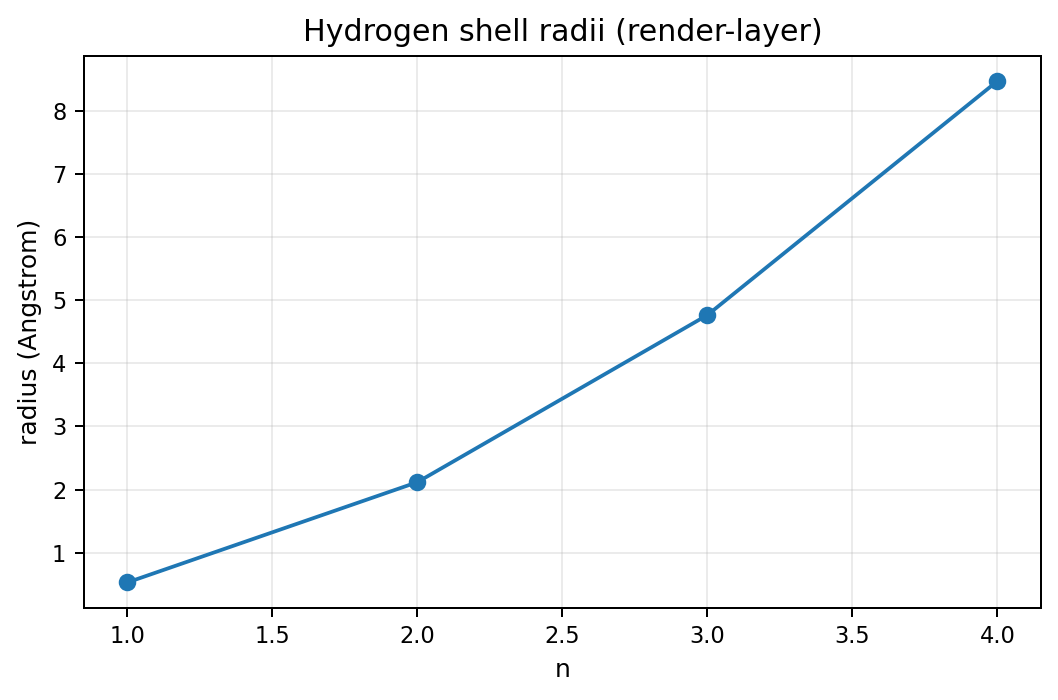
\includegraphics[width=0.74\linewidth]{figures/hydrogen/hydrogen_shell_radii.png}
\caption{Hydrogen shell radii attached after the cited shell row is fixed. The plotted radii are render-layer witnesses only; the cited row remains authoritative.}
\end{figure}

\FloatBarrier

\paragraph{Hook / Evidence.} Use the cited shell-band and attenuation hooks together with the local shell-radius report declared in this section.

\paragraph{Companion notebook and manifest.} See Section~\ref{app:suppc-notebooks} for the executed calculation manifest and generated figure provenance for this section.

\begin{quote}\small\path{notebooks/hydrogen/c4_hydrogen_shell_worked.ipynb}\end{quote}
